% Created by tikzDevice version 0.10.1 on 2016-08-25 15:51:08
% !TEX encoding = UTF-8 Unicode
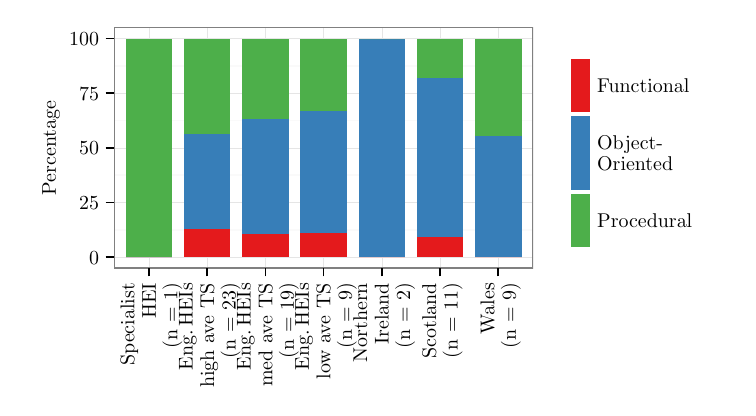
\begin{tikzpicture}[x=1pt,y=1pt]
\definecolor{fillColor}{RGB}{255,255,255}
\path[use as bounding box,fill=fillColor,fill opacity=0.00] (0,0) rectangle (252.94,130.09);
\begin{scope}
\path[clip] (  0.00,  0.00) rectangle (252.94,130.09);
\definecolor{drawColor}{RGB}{255,255,255}
\definecolor{fillColor}{RGB}{255,255,255}

\path[draw=drawColor,line width= 0.6pt,line join=round,line cap=round,fill=fillColor] (  0.00,  0.00) rectangle (252.94,130.09);
\end{scope}
\begin{scope}
\path[clip] ( 31.20, 43.19) rectangle (182.66,130.09);
\definecolor{fillColor}{RGB}{255,255,255}

\path[fill=fillColor] ( 31.20, 43.19) rectangle (182.66,130.09);
\definecolor{drawColor}{gray}{0.98}

\path[draw=drawColor,line width= 0.6pt,line join=round] ( 31.20, 57.02) --
	(182.66, 57.02);

\path[draw=drawColor,line width= 0.6pt,line join=round] ( 31.20, 76.76) --
	(182.66, 76.76);

\path[draw=drawColor,line width= 0.6pt,line join=round] ( 31.20, 96.51) --
	(182.66, 96.51);

\path[draw=drawColor,line width= 0.6pt,line join=round] ( 31.20,116.26) --
	(182.66,116.26);
\definecolor{drawColor}{gray}{0.90}

\path[draw=drawColor,line width= 0.2pt,line join=round] ( 31.20, 47.14) --
	(182.66, 47.14);

\path[draw=drawColor,line width= 0.2pt,line join=round] ( 31.20, 66.89) --
	(182.66, 66.89);

\path[draw=drawColor,line width= 0.2pt,line join=round] ( 31.20, 86.64) --
	(182.66, 86.64);

\path[draw=drawColor,line width= 0.2pt,line join=round] ( 31.20,106.39) --
	(182.66,106.39);

\path[draw=drawColor,line width= 0.2pt,line join=round] ( 31.20,126.14) --
	(182.66,126.14);

\path[draw=drawColor,line width= 0.2pt,line join=round] ( 43.82, 43.19) --
	( 43.82,130.09);

\path[draw=drawColor,line width= 0.2pt,line join=round] ( 64.86, 43.19) --
	( 64.86,130.09);

\path[draw=drawColor,line width= 0.2pt,line join=round] ( 85.90, 43.19) --
	( 85.90,130.09);

\path[draw=drawColor,line width= 0.2pt,line join=round] (106.93, 43.19) --
	(106.93,130.09);

\path[draw=drawColor,line width= 0.2pt,line join=round] (127.97, 43.19) --
	(127.97,130.09);

\path[draw=drawColor,line width= 0.2pt,line join=round] (149.01, 43.19) --
	(149.01,130.09);

\path[draw=drawColor,line width= 0.2pt,line join=round] (170.04, 43.19) --
	(170.04,130.09);
\definecolor{fillColor}{RGB}{228,26,28}

\path[fill=fillColor] ( 35.41, 47.14) rectangle ( 52.24, 47.14);
\definecolor{fillColor}{RGB}{55,126,184}

\path[fill=fillColor] ( 35.41, 47.14) rectangle ( 52.24, 47.14);
\definecolor{fillColor}{RGB}{77,175,74}

\path[fill=fillColor] ( 35.41, 47.14) rectangle ( 52.24,126.14);
\definecolor{fillColor}{RGB}{228,26,28}

\path[fill=fillColor] ( 56.45, 47.14) rectangle ( 73.27, 57.44);
\definecolor{fillColor}{RGB}{55,126,184}

\path[fill=fillColor] ( 56.45, 57.44) rectangle ( 73.27, 91.79);
\definecolor{fillColor}{RGB}{77,175,74}

\path[fill=fillColor] ( 56.45, 91.79) rectangle ( 73.27,126.14);
\definecolor{fillColor}{RGB}{228,26,28}

\path[fill=fillColor] ( 77.48, 47.14) rectangle ( 94.31, 55.46);
\definecolor{fillColor}{RGB}{55,126,184}

\path[fill=fillColor] ( 77.48, 55.46) rectangle ( 94.31, 97.03);
\definecolor{fillColor}{RGB}{77,175,74}

\path[fill=fillColor] ( 77.48, 97.03) rectangle ( 94.31,126.14);
\definecolor{fillColor}{RGB}{228,26,28}

\path[fill=fillColor] ( 98.52, 47.14) rectangle (115.35, 55.92);
\definecolor{fillColor}{RGB}{55,126,184}

\path[fill=fillColor] ( 98.52, 55.92) rectangle (115.35, 99.80);
\definecolor{fillColor}{RGB}{77,175,74}

\path[fill=fillColor] ( 98.52, 99.80) rectangle (115.35,126.14);
\definecolor{fillColor}{RGB}{228,26,28}

\path[fill=fillColor] (119.55, 47.14) rectangle (136.38, 47.14);
\definecolor{fillColor}{RGB}{55,126,184}

\path[fill=fillColor] (119.55, 47.14) rectangle (136.38,126.14);
\definecolor{fillColor}{RGB}{77,175,74}

\path[fill=fillColor] (119.55,126.14) rectangle (136.38,126.14);
\definecolor{fillColor}{RGB}{228,26,28}

\path[fill=fillColor] (140.59, 47.14) rectangle (157.42, 54.32);
\definecolor{fillColor}{RGB}{55,126,184}

\path[fill=fillColor] (140.59, 54.32) rectangle (157.42,111.77);
\definecolor{fillColor}{RGB}{77,175,74}

\path[fill=fillColor] (140.59,111.77) rectangle (157.42,126.14);
\definecolor{fillColor}{RGB}{228,26,28}

\path[fill=fillColor] (161.63, 47.14) rectangle (178.46, 47.14);
\definecolor{fillColor}{RGB}{55,126,184}

\path[fill=fillColor] (161.63, 47.14) rectangle (178.46, 91.03);
\definecolor{fillColor}{RGB}{77,175,74}

\path[fill=fillColor] (161.63, 91.03) rectangle (178.46,126.14);
\definecolor{drawColor}{gray}{0.50}

\path[draw=drawColor,line width= 0.6pt,line join=round,line cap=round] ( 31.20, 43.19) rectangle (182.66,130.09);
\end{scope}
\begin{scope}
\path[clip] (  0.00,  0.00) rectangle (252.94,130.09);
\definecolor{drawColor}{RGB}{0,0,0}

\node[text=drawColor,anchor=base east,inner sep=0pt, outer sep=0pt, scale=  0.72] at ( 25.80, 44.66) {0};

\node[text=drawColor,anchor=base east,inner sep=0pt, outer sep=0pt, scale=  0.72] at ( 25.80, 64.41) {25};

\node[text=drawColor,anchor=base east,inner sep=0pt, outer sep=0pt, scale=  0.72] at ( 25.80, 84.16) {50};

\node[text=drawColor,anchor=base east,inner sep=0pt, outer sep=0pt, scale=  0.72] at ( 25.80,103.91) {75};

\node[text=drawColor,anchor=base east,inner sep=0pt, outer sep=0pt, scale=  0.72] at ( 25.80,123.66) {100};
\end{scope}
\begin{scope}
\path[clip] (  0.00,  0.00) rectangle (252.94,130.09);
\definecolor{drawColor}{RGB}{0,0,0}

\path[draw=drawColor,line width= 0.6pt,line join=round] ( 28.20, 47.14) --
	( 31.20, 47.14);

\path[draw=drawColor,line width= 0.6pt,line join=round] ( 28.20, 66.89) --
	( 31.20, 66.89);

\path[draw=drawColor,line width= 0.6pt,line join=round] ( 28.20, 86.64) --
	( 31.20, 86.64);

\path[draw=drawColor,line width= 0.6pt,line join=round] ( 28.20,106.39) --
	( 31.20,106.39);

\path[draw=drawColor,line width= 0.6pt,line join=round] ( 28.20,126.14) --
	( 31.20,126.14);
\end{scope}
\begin{scope}
\path[clip] (  0.00,  0.00) rectangle (252.94,130.09);
\definecolor{drawColor}{RGB}{0,0,0}

\path[draw=drawColor,line width= 0.6pt,line join=round] ( 43.82, 40.19) --
	( 43.82, 43.19);

\path[draw=drawColor,line width= 0.6pt,line join=round] ( 64.86, 40.19) --
	( 64.86, 43.19);

\path[draw=drawColor,line width= 0.6pt,line join=round] ( 85.90, 40.19) --
	( 85.90, 43.19);

\path[draw=drawColor,line width= 0.6pt,line join=round] (106.93, 40.19) --
	(106.93, 43.19);

\path[draw=drawColor,line width= 0.6pt,line join=round] (127.97, 40.19) --
	(127.97, 43.19);

\path[draw=drawColor,line width= 0.6pt,line join=round] (149.01, 40.19) --
	(149.01, 43.19);

\path[draw=drawColor,line width= 0.6pt,line join=round] (170.04, 40.19) --
	(170.04, 43.19);
\end{scope}
\begin{scope}
\path[clip] (  0.00,  0.00) rectangle (252.94,130.09);
\definecolor{drawColor}{RGB}{0,0,0}

\node[text=drawColor,rotate= 90.00,anchor=base east,inner sep=0pt, outer sep=0pt, scale=  0.72] at ( 38.53, 37.79) {Specialist};

\node[text=drawColor,rotate= 90.00,anchor=base east,inner sep=0pt, outer sep=0pt, scale=  0.72] at ( 46.30, 37.79) {HEI};

\node[text=drawColor,rotate= 90.00,anchor=base east,inner sep=0pt, outer sep=0pt, scale=  0.72] at ( 54.08, 37.79) {(n = 1)};

\node[text=drawColor,rotate= 90.00,anchor=base east,inner sep=0pt, outer sep=0pt, scale=  0.72] at ( 59.56, 37.79) {Eng.\,HEIs};

\node[text=drawColor,rotate= 90.00,anchor=base east,inner sep=0pt, outer sep=0pt, scale=  0.72] at ( 67.34, 37.79) {high ave TS};

\node[text=drawColor,rotate= 90.00,anchor=base east,inner sep=0pt, outer sep=0pt, scale=  0.72] at ( 75.12, 37.79) {(n = 23)};

\node[text=drawColor,rotate= 90.00,anchor=base east,inner sep=0pt, outer sep=0pt, scale=  0.72] at ( 80.60, 37.79) {Eng.\,HEIs};

\node[text=drawColor,rotate= 90.00,anchor=base east,inner sep=0pt, outer sep=0pt, scale=  0.72] at ( 88.38, 37.79) {med ave TS};

\node[text=drawColor,rotate= 90.00,anchor=base east,inner sep=0pt, outer sep=0pt, scale=  0.72] at ( 96.15, 37.79) {(n = 19)};

\node[text=drawColor,rotate= 90.00,anchor=base east,inner sep=0pt, outer sep=0pt, scale=  0.72] at (101.64, 37.79) {Eng.\,HEIs};

\node[text=drawColor,rotate= 90.00,anchor=base east,inner sep=0pt, outer sep=0pt, scale=  0.72] at (109.41, 37.79) {low ave TS};

\node[text=drawColor,rotate= 90.00,anchor=base east,inner sep=0pt, outer sep=0pt, scale=  0.72] at (117.19, 37.79) {(n = 9)};

\node[text=drawColor,rotate= 90.00,anchor=base east,inner sep=0pt, outer sep=0pt, scale=  0.72] at (122.67, 37.79) {Northern};

\node[text=drawColor,rotate= 90.00,anchor=base east,inner sep=0pt, outer sep=0pt, scale=  0.72] at (130.45, 37.79) {Ireland};

\node[text=drawColor,rotate= 90.00,anchor=base east,inner sep=0pt, outer sep=0pt, scale=  0.72] at (138.22, 37.79) {(n = 2)};

\node[text=drawColor,rotate= 90.00,anchor=base east,inner sep=0pt, outer sep=0pt, scale=  0.72] at (147.60, 37.79) {Scotland};

\node[text=drawColor,rotate= 90.00,anchor=base east,inner sep=0pt, outer sep=0pt, scale=  0.72] at (155.37, 37.79) {(n = 11)};

\node[text=drawColor,rotate= 90.00,anchor=base east,inner sep=0pt, outer sep=0pt, scale=  0.72] at (168.63, 37.79) {Wales};

\node[text=drawColor,rotate= 90.00,anchor=base east,inner sep=0pt, outer sep=0pt, scale=  0.72] at (176.41, 37.79) {(n = 9)};
\end{scope}
\begin{scope}
\path[clip] (  0.00,  0.00) rectangle (252.94,130.09);
\definecolor{drawColor}{RGB}{0,0,0}

\node[text=drawColor,rotate= 90.00,anchor=base,inner sep=0pt, outer sep=0pt, scale=  0.72] at ( 10.20, 86.64) {Percentage};
\end{scope}
\begin{scope}
\path[clip] (  0.00,  0.00) rectangle (252.94,130.09);
\definecolor{fillColor}{RGB}{255,255,255}

\path[fill=fillColor] (191.20, 45.91) rectangle (244.41,127.37);
\end{scope}
\begin{scope}
\path[clip] (  0.00,  0.00) rectangle (252.94,130.09);
\definecolor{fillColor}{RGB}{228,26,28}

\path[fill=fillColor] (196.18, 99.69) rectangle (203.29,118.77);
\end{scope}
\begin{scope}
\path[clip] (  0.00,  0.00) rectangle (252.94,130.09);
\definecolor{fillColor}{RGB}{55,126,184}

\path[fill=fillColor] (196.18, 71.40) rectangle (203.29, 98.26);
\end{scope}
\begin{scope}
\path[clip] (  0.00,  0.00) rectangle (252.94,130.09);
\definecolor{fillColor}{RGB}{77,175,74}

\path[fill=fillColor] (196.18, 50.89) rectangle (203.29, 69.98);
\end{scope}
\begin{scope}
\path[clip] (  0.00,  0.00) rectangle (252.94,130.09);
\definecolor{drawColor}{RGB}{0,0,0}

\node[text=drawColor,anchor=base west,inner sep=0pt, outer sep=0pt, scale=  0.72] at (205.81,114.53) {};

\node[text=drawColor,anchor=base west,inner sep=0pt, outer sep=0pt, scale=  0.72] at (205.81,106.75) {Functional};

\node[text=drawColor,anchor=base west,inner sep=0pt, outer sep=0pt, scale=  0.72] at (205.81, 98.98) {};
\end{scope}
\begin{scope}
\path[clip] (  0.00,  0.00) rectangle (252.94,130.09);
\definecolor{drawColor}{RGB}{0,0,0}

\node[text=drawColor,anchor=base west,inner sep=0pt, outer sep=0pt, scale=  0.72] at (205.81, 94.02) {};

\node[text=drawColor,anchor=base west,inner sep=0pt, outer sep=0pt, scale=  0.72] at (205.81, 86.24) {Object-};

\node[text=drawColor,anchor=base west,inner sep=0pt, outer sep=0pt, scale=  0.72] at (205.81, 78.46) {Oriented};

\node[text=drawColor,anchor=base west,inner sep=0pt, outer sep=0pt, scale=  0.72] at (205.81, 70.69) {};
\end{scope}
\begin{scope}
\path[clip] (  0.00,  0.00) rectangle (252.94,130.09);
\definecolor{drawColor}{RGB}{0,0,0}

\node[text=drawColor,anchor=base west,inner sep=0pt, outer sep=0pt, scale=  0.72] at (205.81, 65.73) {};

\node[text=drawColor,anchor=base west,inner sep=0pt, outer sep=0pt, scale=  0.72] at (205.81, 57.95) {Procedural};

\node[text=drawColor,anchor=base west,inner sep=0pt, outer sep=0pt, scale=  0.72] at (205.81, 50.18) {};
\end{scope}
\end{tikzpicture}
